\documentclass{beamer}
\usepackage[latin1]{inputenc}

%\usepackage[noend]{algpseudocode}
%\usepackage[ruled]{algorithm}
\usepackage{url}
\usepackage{framed}
\usepackage{amsfonts,amsmath,amsthm}
\usepackage{graphicx}
\usepackage{url}
\usepackage{color}

\usepackage[english]{babel}

% font definitions, try \usepackage{ae} instead of the following
% three lines if you don't like this look
\usepackage[scaled=.90]{helvet}
\usepackage{courier}
\usepackage{mathptmx}
\usepackage{pgf}
\usepackage{tikz}
\usetikzlibrary{snakes,arrows,shapes,patterns,positioning,shapes.misc,shapes.geometric,shapes.callouts,decorations.text}
\usepackage[ruled,vlined,linesnumbered]{algorithm2e}

\title{Rational Metareasoning in Problem-Solving Search}
\author{David Tolpin}
\institute{Ben-Gurion University of the Negev\\Beer Sheva, Israel}
\date{February 12, 2014}

%%%----------------------------
\def\defemb#1#2{\expandafter\def\csname #1\endcsname
                              {\relax\ifmmode #2\else\hbox{$#2$}\fi}}
\defemb{cA}{{\cal A}}
\defemb{cB}{{\cal B}}
\defemb{cC}{{\cal C}}
\defemb{cc}{{\cal c}}
\defemb{cD}{{\cal D}}
\defemb{cE}{{\cal E}}
\defemb{cF}{{\cal F}}
\defemb{cf}{{\cal f}}
\defemb{cv}{{\cal v}}
\defemb{cx}{{\cal x}}

\defemb{cG}{{\cal G}}
\defemb{GG}{{\cal G}}

\defemb{cI}{{\cal I}}
\defemb{cK}{{\cal K}}
\defemb{cP}{{\cal P}}
\defemb{cL}{{\cal L}}
\defemb{cN}{{\cal N}}
\defemb{cM}{{\cal M}}
\defemb{cR}{{\cal R}}

\defemb{cS}{{\cal S}}
\defemb{SS}{{\cal S}}

\defemb{cT}{{\cal T}}
\defemb{cV}{{\cal V}}
\defemb{cU}{{\cal U}}
\defemb{cO}{{\cal O}}
\defemb{cH}{{\cal H}}
\defemb{cX}{{\cal X}}
\defemb{cY}{{\cal Y}}
\defemb{cZ}{{\cal Z}}

\defemb{sP}{{\sf P}}
\defemb{sG}{{\sf G}}
\defemb{sU}{{\sf U}}
\defemb{sE}{{\sf E}}
\defemb{sI}{{\sf I}}
\defemb{su}{{\sf u}}
\defemb{se}{{\sf e}}
\defemb{ss}{{\sf s}}
\defemb{st}{{\sf t}}
\defemb{sp}{{\sf p}}
\defemb{si}{{\sf i}}
\defemb{sb}{{\sf b}}
\defemb{sw}{{\sf w}}
\defemb{sA}{{\sf A}}
\defemb{sB}{{\sf B}}
\defemb{sa}{{\sf a}}
\defemb{sb}{{\sf b}}
\defemb{scc}{{\sf c}}
\defemb{sd}{{\sf d}}



\defemb{tta}{{\tt a}}
\defemb{ttb}{{\tt b}}
\defemb{ttc}{{\tt c}}
\defemb{ttd}{{\tt d}}
\defemb{tte}{{\tt e}}
\defemb{ttf}{{\tt f}}

\defemb{bara}{{\bar{a}}}
\defemb{barb}{{\bar{b}}}
\defemb{barc}{{\bar{c}}}
\defemb{barf}{{\bar{f}}}
\defemb{barv}{{\bar{v}}}


\newcommand{\argmax}{\operatornamewithlimits{argmax}}
\newcommand{\argmin}{\operatornamewithlimits{argmin}}



\newtheorem{proposition}{Proposition}
\newtheorem{cor}{Corollary}
\newtheorem{notation}{Notation}


\newcommand{\domainname}[1]{{\footnotesize{\textsc{#1}}}}
\newcommand{\domainnamess}[1]{{\scriptsize{\textsc{#1}}}}

\def\reals{{\mathbb R}}
\def\nat{{\mathbb N}}
\def\natplus{{\mathbb N^{+}}}
\newcommand{\nnreals}{\reals^{0+}}
\newcommand{\eqbydef}{\stackrel{{\mathsf{def}}}{=}}

\newcommand{\strips}{\textsc{strips}}
\newcommand{\nstrips}{\textsc{ub}}
\newcommand{\sas}{\textsc{sas}${}^{+}$}
%\newcommand{\prj}[2]{#1|_{#2}}
\newcommand{\prj}[2]{#1\ptrnabst{#2}}


\newcommand{\pdomain}{\cD}
\newcommand{\nindex}[1]{_{#1}}
\newcommand{\alphafactor}[2]{\alpha(#1,#2)}
%\newcommand{\alphafactor}[2]{\alpha_{(#1,#2)}}
\newcommand{\cconst}[2]{\alphafactor{#1}{#2}}

\newcommand{\indegree}{\mathsf{In}}
\newcommand{\outdegree}{\mathsf{Out}}
\newcommand{\treeclass}{{\mathbf{T}}}
\newcommand{\itreeclass}{{\mathbf{I}}}
\newcommand{\ptreeclass}{{\mathbf{P}}}
\newcommand{\singlyclass}{{\mathbf{S}}}
\newcommand{\climit}{b}
\newcommand{\ilimit}{_{\climit}}
\newcommand{\olimit}{^{\climit}}
\newcommand{\edge}{e}
\newcommand{\elabel}[2]{\|#1,#2\|}
\newcommand{\descendants}{{\mathsf{Desc}}}
\newcommand{\deplimit}[1]{\mbox{\sl db}_{#1}}


\newcommand{\fdecomposition}{$\EuScript{F}$-decomposition}
\newcommand{\idecomposition}{$\EuScript{I}$-decomposition}
\newcommand{\fidecomposition}{$\EuScript{FI}$-decomposition}

\newcommand{\leftq}{\llbracket}
\newcommand{\rightq}{\rrbracket}

\newcommand{\bound}{b}

\newcommand{\statemodel}{\cS}
\newcommand{\state}{s}
\newcommand{\states}{S}
\newcommand{\initstate}{\state_{0}}
\newcommand{\goalstates}{\states_{\goal}}
\newcommand{\transfunc}{f}
\newcommand{\appactions}[1]{\actions(#1)}
\newcommand{\actionSeq}{\plan}
\newcommand{\actionSeqs}{A^{\ast}}
\newcommand{\tind}[1]{_{#1}}

%\newcommand{\costfunc}{{\sl cost}}
\newcommand{\costfunc}{\cC}
\newcommand{\liftcostfunc}{C}
\newcommand{\optcost}{C^\ast}
\newcommand{\treecost}{\sigma}
\newcommand{\intercost}{M}
\newcommand{\localcost}{L}
\newcommand{\result}{Result}
\newcommand{\vchanges}[2]{{\mathrm{vc}}(#1,#2)}
\newcommand{\eff}{{\mathsf{eff}}}
\newcommand{\prv}{{\mathsf{prv}}}
\newcommand{\pre}{{\mathsf{pre}}}
\newcommand{\post}{{\mathsf{post}}}
\newcommand{\actions}{A}
\newcommand{\cost}{Cost}
\newcommand{\totalcost}{\textbf{Cost}}
\newcommand{\costs}{C}
\newcommand{\parent}{Pa}
\newcommand{\children}{Ch}
\newcommand{\before}[2]{{#1}_{#2}}
\newcommand{\domain}{dom}

\newcommand{\copprob}{{\sf COP}}
\newcommand{\copvars}{\cX}
\newcommand{\copvarsvars}{\cX^{\vars}}
\newcommand{\copvarsedges}{\cX^{\cE}}
\newcommand{\copvar}{x}
\newcommand{\copfuncs}{\cF}
\newcommand{\copscope}{Q}
\newcommand{\copf}{\varphi}

\newcommand{\prefixes}[1]{\unrhd[#1]}
\newcommand{\vprefixes}[1]{\unrhd^{\ast}[#1]}
\newcommand{\postfixes}[1]{\unlhd[#1]}

\newcommand{\actionone}[1]{\action_{#1}}
\newcommand{\actiontwo}[2]{\action_{#1|#2}}
\newcommand{\costone}[1]{C_{#1}}
\newcommand{\costtwo}[2]{C_{#1|#2}}

\newcommand{\treewidth}{w}
%\newcommand{\causalG}[1]{\mbox{\sl CG}_{#1}}
\newcommand{\cgedges}{E}
\newcommand{\causalG}[1]{\mbox{\sl CG}({#1})}
\newcommand{\cgsp}{\cG}
\newcommand{\cgspset}{{\mathbf{G}}}
\newcommand{\dtG}[2]{\mbox{\sl DTG}(#1,#2)}
%\newcommand{\ucausalG}[1]{\overline{\mbox{\sl CG}}_{#1}}
\newcommand{\ucausalG}[1]{\mbox{\sl G}_{CG}}
%\newcommand{\darc}[2]{(\overrightarrow{#1, #2})}
\newcommand{\darc}[2]{(#1, #2)}
\newcommand{\uarc}[2]{(#1, #2)}

%\newcommand{\init}{I}
\newcommand{\init}{\initstate}
\newcommand{\goal}{G}
\newcommand{\troot}{r}
\newcommand{\tree}{T}
\newcommand{\vars}{V}
\newcommand{\varsset}{\cV}
\newcommand{\probset}{{\mathbf{\Pi}}}
\newcommand{\laction}[3]{\action_{#1}^{#3|#2}}
\newcommand{\ilaction}[4]{A_{#2|#1}^{#4|#3}}
\newcommand{\lcost}[3]{\costs_{#1}^{#3|#2}}
\newcommand{\ilcost}[4]{\costs_{#2|#1}^{#4|#3}}
\newcommand{\dummyroot}{\hat{\troot}}
\newcommand{\plan}{\rho}
\newcommand{\oplan}{\overline{\plan}}

%%%%%%%%%%%%%%%%%%%%%%%%%%%%%%%%%%%%%%%%%%%%%%%%%%%%%%%%%%%%%%%%%%%%%%%%%%%%%%%%%%%
%%%%%%%%%%%%%% from jair 2003 %%%%%%%%%%%%%%%%%%%%%%%%%%%%%%%%%%%%%%%%%%%%%%%%%%%%%
%% Planning
%% --------

\newenvironment{atheorem}[1]{{\vspace{0.4cm}\noindent\bf Theorem~\ref{#1}}~~}
                            {\\}
\newenvironment{alemma}[1]{{\vspace{0.4cm}\noindent\bf Lemma~\ref{#1}}~~}
                            {\\}


\newcommand{\sset}[1]{
  \left\{ \begin{array}{l}#1\end{array} \right.}


%\newcommand{\scite}{\citeyear}
\newcommand{\proofsout}[1]{}
\newcommand{\commentout}[1]{}
\newcommand{\journal}[1]{}
\newcommand{\conference}[1]{#1}

\newcommand{\parents}{{\mathsf{pred}}}
\newcommand{\sons}{{\mathsf{succ}}}
\newcommand{\lparents}{pred}
\newcommand{\lsons}{succ}
\newcommand{\plans}{{\mathbf\Pi}}
\newcommand{\allsons}{AllSucc}

\newcommand{\Can}{{\mathsf{MaxPoss}}}
\newcommand{\newCan}{{\mathsf{newMaxPoss}}}
\newcommand{\FeasibleMust}{{\mathsf{FMaxReq}}}
\newcommand{\Must}{{\mathsf{MaxReq}}}
\newcommand{\LocalMust}{{\mathsf{Req}}}
\newcommand{\newMust}{{\mathsf{newMaxReq}}}
\newcommand{\minplan}{{\mathsf{MinPlanSize}}}
\newcommand{\maxplan}{{\mathsf{MaxPlanSize}}}

%\newcommand{\fdec}{{\EuScript{F}}}
%\newcommand{\idec}{{\EuScript{I}}}
%\newcommand{\fidec}{{\EuScript{F\!I}}}
%\newcommand{\ifdec}{\idec}
\newcommand{\fdec}{^{\mathsf{f}}}
\newcommand{\idec}{^{\mathsf{i}}}
\newcommand{\fidec}{^{\mathsf{fi}}}
\newcommand{\ifdec}{\idec}

\newcommand{\Fdec}{{\EuScript{F}}}
\newcommand{\Idec}{{\EuScript{I}}}
\newcommand{\FIdec}{{\EuScript{F\!I}}}



\newcommand{\truecost}{h^{\ast}}
\newcommand{\hplus}{h^{+}}
\newcommand{\hK}{h^{k}}
\newcommand{\hpdb}{h^{\text{PDB}}}
\newcommand{\hapdb}{h^{\text{PDB}}_{\text{add}}}



%\newcommand{\ahfork}{h_{{}_{\merge}}}
\newcommand{\ahfi}{h^{\FIdec}}
\newcommand{\ahf}{h^{\Fdec}}
\newcommand{\ahi}{h^{\Idec}}
\newcommand{\ahfork}{\ahfi}


\newcommand{\hff}{h_{\mathrm{FF}}}
\newcommand{\hffgen}{h_{\mathrm{ff}}}
\newcommand{\hplusone}{h^{+s}}
\newcommand{\hadd}{h_{{\mathrm{add}}}}
\newcommand{\ahmax}{h_{{\mathrm{max}}}}
\newcommand{\ahm}[1]{h^{#1}}
\newcommand{\ahsum}[1]{h^{#1}_{{}_{\sum}}}


\newcommand{\ptrnabst}[1]{^{[ #1 ]}}
\newcommand{\pattern}{\vars'}
\newcommand{\ahsp}{h_{{\mathrm{sp}}}}
\newcommand{\actsequence}{\varrho}
\newcommand{\odplans}{\cP^{\textrm{c}}}

\newcommand{\sequence}{\sigma}

\newcommand{\condsubplan}[4]{\hat{#4}_{#1_{#2}}^{#3}}
\newcommand{\condsubplanl}[3]{\hat{l}_{#1_{#2}}^{#3}}
\newcommand{\condsubplanp}[3]{\hat{p}_{#1_{#2}}^{#3}}
%boolean for uniform-cost
\newcommand{\condsubplanb}[3]{\hat{\delta}_{#1_{#2}}^{#3}}
\newcommand{\condsubplansigma}[2]{\hat{n}_{#1}^{#2}}


\newcommand{\Ocondsubplan}[3]{\plan_{#1_{#2}}^{#3}}
\newcommand{\Ocondsubplanl}[3]{l_{#1_{#2}}^{#3}}
\newcommand{\Ocondsubplanp}[3]{p_{#1_{#2}}^{#3}}
%boolean for uniform-cost
\newcommand{\Ocondsubplanb}[3]{\delta_{#1_{#2}}^{#3}}
\newcommand{\Ocondsubplansigma}[2]{n_{#1}^{#2}}

\newcommand{\COPcondsubplan}[3]{\Ocondsubplan{#1}{#2}{#3}}
\newcommand{\COPcondsubplanl}[3]{\Ocondsubplanl{#1}{#2}{#3}}
\newcommand{\COPcondsubplanp}[3]{\Ocondsubplanp{#1}{#2}{#3}}
%boolean for uniform-cost
\newcommand{\COPcondsubplanb}[3]{\Ocondsubplanb{#1}{#2}{#3}}
\newcommand{\COPcondsubplansigma}[2]{n_{#1}^{#2}}


\newcommand{\val}{\vartheta}
%\newcommand{\val}{d}
\newcommand{\POP}{{\sc pop-pcg}}

\def\nat{{\mathbb N}}
\def\natzero{{\mathbb N}^{0}}
%\newcommand{\var}{\upsilon}
\newcommand{\var}{v}

\newcommand{\proj}[2]{#1\!\!\!\downarrow_{#2}}
%%%%%%%%%%%%%%%%%%%%%%%%%%%%%%%%%%%%%%%%%%%%%%%%%%%%%%%%%%%%%%%%%%%%%%%%%%%%%%%%%%555

\newcommand{\removed}[1]{}

\newcommand{\carmel}[1]{
  {\footnotesize
  \begin{center}
  \fbox{
    \begin{minipage}{3in}
      carmel: #1
    \end{minipage}
    }
  \end{center}
  }
}





%%% Landmarks

\newcommand{\LMordering}[2]{#1\rightarrow#2}
\newcommand{\LMlocal}{\text{LM}^{\text{local}}}
\newcommand{\LAMA}{\text{LAMA}}
\newcommand{\astarstar}{\text{\it A}^{\ast\ast}}
\newcommand{\astar}{\text{\it A}^{\ast}}
\newcommand{\bfstar}{\text{\it BF}^{\ast}}
\newcommand{\facts}{F}
\newcommand{\varfact}{\psi}
%\newcommand{\LMbfstar}{\text{\it LM-BF}^{\ast}}
\newcommand{\applied}[1]{\leftq #1 \rightq}

%\newcommand{\LMstruct}[1]{\langle \LMs^{#1}, \Nords^{#1}, \NEords^{#1}, \GNEords^{#1} \rangle}
\newcommand{\LMs}{L}
\newcommand{\Nords}{Na}
\newcommand{\NEords}{N}
\newcommand{\GNEords}{GN}
\newcommand{\Reached}[2]{\mathsf{Accepted}(#1,#2)}
\newcommand{\Needed}[2]{\mathsf{ReqAgain}(#1,#2)}

%%% EREZ
\newcommand{\pdastar}{\text{\it PD-A}^{\ast}}
\newcommand{\mpdastar}{\text{\it LM-A}^{\ast}}
%\newcommand{\mpdastar}{\text{\it MPD-A}^{\ast}}
\newcommand{\slist}[1]{\text{\it #1}}
\newcommand{\openlist}{\slist{OPEN}}
\newcommand{\closedlist}{\slist{CLOSED}}
\newcommand{\node}[1]{\begin{it}#1\end{it}}
\newcommand{\f}{f}
\newcommand{\g}{g}
\newcommand{\h}{h}
\newcommand{\fof}[1]{\f(#1)}
\newcommand{\gof}[1]{\g(#1)}
\newcommand{\hof}[1]{\h(#1)}
\newcommand{\lmcost}{cost}
\newcommand{\lmsetcost}{cost}
\newcommand{\almcost}{cost}
\newcommand{\lm}{\fact}
\newcommand{\achievers}{\mathsf{ach}}
\newcommand{\firstachievers}{\mathsf{first-ach}}
\newcommand{\possibleachievers}{\mathsf{possible-ach}}
\newcommand{\hl}{h_L}
\newcommand{\hla}{h_{LA}}
\newcommand{\planproof}{P}
\newcommand{\planproofu}{\planproof_U}
\newcommand{\lmof}{lm}
\newcommand{\LMof}[2]{\LMs(#1|#2)}
\newcommand{\atom}{p}
\newcommand{\varatom}{q}
\newcommand{\UALM}{U}
\newcommand{\LMU}{\LMs_U}
\newcommand{\multipaths}{\mathcal{P}}
%\newcommand{\hhh}{LFPA}
\newcommand{\hhh}{\textit{FA}}
\newcommand{\maxh}{max}
\newcommand{\timeshort}{{\it time}}
\newcommand{\expandedshort}{{\it nodes}}


\newcommand{\fd}{Fast Downward}
\newcommand{\LMstruct}[1]{\langle \LMs^{#1}, \LMords^{#1} \rangle}
\newcommand{\LMords}{Ord}

\newcommand{\PDDL}{\textsc{pddl}}
\newcommand{\pspacehard}{P-SPACE Hard}
\newcommand{\pspacecomplete}{P-SPACE Complete}
\newcommand{\nphard}{NP Hard}
\newcommand{\npcomplete}{NP Complete}
\newcommand{\lmcut}{\h_{\text{LM-CUT}}}
\newcommand{\smaxi}{$\mathrm{sel}_{h}$}
\newcommand{\smaxu}{$\mathrm{sel}_{h}^{U}$}
\newcommand{\randmax}{$\mathrm{rnd}_{h}$}
\newcommand{\smaxzero}{$\mathrm{sel}_{h}^{0}$}
\newcommand{\regmax}{$\max_{h}$}
\newcommand{\best}{$\mathrm{best}$}
%\newcommand{\smaxi}{S-MAX-I}
%\newcommand{\smaxu}{S-MAX-U}
%\newcommand{\randmax}{R-MAX}
%\newcommand{\regmax}{MAX}
\newcommand{\goaldepth}{c^\ast}


\newcommand{\OPEN} {{\textsc{Open}}}
\newcommand{\CLOSED} {{\textsc{Closed}}}
\newcommand{\lazyastar} {\ensuremath{LA^\ast}}
\newcommand{\rationallazyastar} {\ensuremath{RLA^\ast}}
\newcommand{\astarmax}{\ensuremath{\astar_{MAX}}}

\newcommand{\win}[1]{
  \begin{scope}[shift={#1}]
    \begin{scope}[scale=0.25]
      \draw [very thick,draw=green!50!black,fill=green]
            (0,0) .. controls (1.5,-0.5) and (1,-2.0) .. (0,-3)
                  .. controls (0.25, -2) and (-2, -1.5) .. (0,0);
      \draw [thin] (0,0) .. controls (0,-1) and (0.5,-2) .. (0,-3);
    \end{scope}
  \end{scope}}
 
\newcommand{\loss}[1]{
  \begin{scope}[shift={#1}]
    \begin{scope}[scale=0.25]
      \draw [very thick,draw=brown,fill=yellow!50!brown]
            (0,0) .. controls (-1.0,-0.5) and (-0.35,-2.0) .. (0,-3)
                  .. controls (-1.25, -1.75) and (1, -1.5) .. (0,0);
      \draw [thin] (0,0) .. controls (0,-1) and (-0.75,-2) .. (0,-3);
    \end{scope}
  \end{scope}}
  
\AtBeginSection[]
{
  \begin{frame}<beamer>
    \frametitle{Outline}
    \tableofcontents[currentsection]
  \end{frame}
}


\begin{document}

\begin{frame}
\titlepage
\end{frame}

\begin{frame}
\frametitle{Rational Metareasoning in Problem-Solving Search}
\begin{description}
\item[Problem-Solving Search:] \hfill\\ Search time depends dramatically on
  problem instance features other than problem size.
\item[(Limited) Rationality:] \hfill\\ The agent acts to maximize its reward given
  limited resources.
\item[Metareasoning:] \hfill\\ Reasoning about computations which help to
  choose the best action.
\end{description}
\end{frame}

\begin{frame}
\tableofcontents
\end{frame}

\section{Rational Metareasoning}

\begin{frame}{Rational Metareasoning}
\begin{itemize}
\item A problem-solving agent can perform {\it base-level} actions from a known
          set $\{A_i\}$.
\item Before committing to an action, the agent may perform a sequence of
          {\it meta-level} deliberation actions from a set $\{S_j\}$.
\item At any given time there is a base-level action $A_\alpha$ that maximizes
          the agent's {\it expected utility.}
\end{itemize}

          The {\bf net VOI $V(S_j)$} of action $S_j$ is the {\bf intrinsic VOI} $\Lambda_j$ less the cost of $S_j$:
          \[V(S_j)=\Lambda(S_j)-C(S_j)\]
           \[\Lambda(S_j)=\mathbb{E}\left(\mathbb{E}(U(A_\alpha^j))-\mathbb{E}(U(A_\alpha))\right)\]

\begin{itemize} 
\item  $S_{j_{\max}}$ that maximizes the net VOI  is performed: $j_{\max} = \arg\max_jV(S_j)$, if $V(S_{j_{\max}})>0$.
\item Otherwise, $A_\alpha$ is performed.
\end{itemize}
\end{frame}

\begin{frame}
\frametitle{Simplifying assumptions}
\begin{itemize}
\item {\bf Myopicity:}
  \begin{itemize}
  \item Meta-greedy: consider only the effect of single computatitonal actions.
  \item Single-step: Assume all computations are complete, act as
    though a base-level action immediately follows the computation.
  \end{itemize}
\item {\bf Subtree independence:} any computation updates the expected
  utility of a single action.
\end{itemize}
\end{frame}
  
\section{Rational Deployment of Heuristics in CSP}

\begin{frame}{Constraint Satisfaction}
\begin{itemize}
\item CSP backtracking search algorithms typically employ
  variable-ordering and value-ordering heuristics.
\item Many value ordering heuristics are computationally
  heavy, e.g. heuristics {\it based on solution count
          estimates.}
\item Principles of rational metareasoning can be applied
          to decide when to deploy the heuristics.
\end{itemize}
\end{frame}

\begin{frame}{Constraint Satisfaction}
A constraint satisfaction problem (CSP) is defined by:
\begin{itemize}
\item[] {\bf variables} $\mathcal{X}=\{X_1, X_2, ...\}$, 
\item[] {\bf constraints} $\mathcal{C}=\{C_1, C_2, ...\}$. 
\end{itemize}
\begin{itemize}
 \item Each {\it variable} $X_i$ has a non-empty domain
          $D_i$ of possible values. 
\item Each {\it constraint} $C_i$ involves some subset
          of the variables---the {\it scope} of the constraint---and specifies the
          allowable combinations of values for that subset. 
\item An {\it assignment} that does not violate any constraints is called
          {\it consistent} (or solution).
 \end{itemize}
 \end{frame}

\begin{frame}{Value Ordering Model}
Value ordering heuristics provide information about:
\begin{itemize}
 \item $T_i$---the expected time to find a solution containing
          an assignment  $X_k=y_{ki};$
\item $p_i$---the probability that there is no solution
  consistent with $X_k=y_{ki}$.
\end{itemize}
The expected remaining search time in the subtree under $X_k$ for
ordering $\omega$ is $T^{s|\omega}=T_{\omega(1)}+\sum_{i=2}^{|D_k|}T_{\omega(i)}\prod_{j=1}^{i-1}p_{\omega(j)}$
\begin{itemize}
\item The current optimal base-level action is picking the $\omega $ which optimizes $T^{s|\omega}$.  $T^{s|\omega}$ is minimal if the values are sorted  by increasing order of $\frac {T_i} {1-p_i}$.
\item The intrinsic VOI $\Lambda_i$ of estimating $T_i, p_i$ for the $i$th assignment is the expected decrease in the expected search time:
          $\Lambda_i=\mathbb{E}\left[T^{s|\omega_-}-T^{s|\omega_{+i}}\right]$.
\end{itemize}
\end{frame}

\begin{frame}
\frametitle{Model Assumptions}

\begin{enumerate}
\item Solutions are roughly evenly distributed in the search space, that is,
   the distribution of time to find a solution can be modeled by a
   Poisson process.
\item Finding all solutions for an assignment $X_{k}=y_{ki}$
takes roughly the same time for all assignments to the variable $X_k$.
\item The expected time to find all solutions for an assignment
  divided by its solution count estimate is a
  reasonable estimate for the expected time to find a single solution. 
\end{enumerate}
\end{frame}


\begin{frame}{Main Results}

{\large{\bf Rational Value Ordering}}

The intrinsic VOI $\Lambda_i$ of invoking the heuristic can be approximated as:
\[\Lambda_i\approx \mathbb{E}\left[(T_1-T_i)|D_k|\,\Big|\; T_i < T_1 \right]\]

{\large{\bf VOI of Solution Count Estimates}}

The net VOI $V$ of estimating a solution count can be approximated as:
\[V \propto |D_k|e^{-\nu}\sum_{n=n_\mathrm{max}}^\infty \! \! \left( \frac 1 {n_\mathrm{max}} - \frac 1 n\right) \frac {\nu^n} {n!}-\gamma\]
where the constant $\gamma$ \textcolor{blue}{depends on the search algorithm and the heuristic, rather than on the CSP instance,} and can be learned offline. 
\end{frame}

\begin{frame}{Benchmarks}
\vspace{-24pt}
\begin{figure}[h]
\centering
\includegraphics[scale=0.6]{benchmarks.pdf}

14 CSP Solver Competion 2005 Benchmarks\\
solved for $\gamma \in \{0, 10^{-7},$ $10^{-6},$ $...,$ $1\}$
\end{figure}
\end{frame}


\begin{frame}{Random Instances}
\begin{figure}[h] 
\centering
\includegraphics[scale=0.6]{random-problems-arrows+legend.pdf}

100 Model RB Random Instances
\end{figure}
\end{frame}

\begin{frame}{Generalized Sudoku}
\begin{itemize}
\item Real-world problem instances often have much more structure
  than random instances generated according to Model RB.
\item We repeated the
  experiments on randomly generated Generalized Sudoku instances---
  a highly structured domain.
\item Relative performance on Generalized Sudoku was similar to
  Model~RB.
\end{itemize}
\end{frame}

\section{VOI-aware Monte Carlo Tree Search}

\begin{frame}{MCTS}

{\bf M}onte {\bf C}arlo {\bf T}ree {\bf S}earch helps in large search spaces.At each node:
\begin{itemize}
\item Repeats:
  \begin{enumerate}
    \item \textbf{Selection:} select an action to explore.
    \item \textbf{Simulation:} simulates a rollout until a goal is reached.
    \item \textbf{Backpropagation:} updates the action value.
  \end{enumerate}
\item Selects the best action.
\end{itemize}
\vspace{1em}
\textbf{Adaptive} Generally, MCTS samples `good' moves more frequently,\\
but sometimes {\bf explores} new directions.
\end{frame}

\begin{frame}{Multi-armed Bandit Problem and UCB}
Multi-armed Bandit Problem:
\begin{itemize}
\item We are given a set of $K$ arms.
\item Each arm can be pulled multiple times.
\item The reward is drawn from an {\bf unknown} (but normally {\it
    stationary} and {\it bounded}) distribution.
\item The {\bf total reward} must be maximized.
\end{itemize}

{\bf UCB} is near-optimal for MAB --- solves
{\it exploration/exploitation} tradeoff.
\begin{itemize}
\item pulls an arm that maximizes {\bf U}pper {\bf C}onfidence {\bf
    B}ound: $b_i=\overline X_i+\sqrt {\frac {c \log (n)} {n_i}}$
\item the cumulative regret is $O(\log n)$.
\end{itemize}
\end{frame}

\begin{frame}{UCT}
UCT ({\bf U}pper {\bf C}onfidence Bounds applied to {\bf T}rees) is 
based on UCB.
\begin{itemize}
\item Adaptive MCTS.
\item Applies the UCB selection scheme at each step of the rollout.
\item Demonstrated good performance in Computer Go (MoGo, CrazyStone, Fuego,
  Pachi, ...) as well as in other domains.
\end{itemize}
However, the first step of a rollout is different:
\begin{itemize}
\item The purpose of MCTS is to choose an action with the greatest utility.
\item Therefore, the {\bf simple regret} must be minimized.
\end{itemize}
\end{frame}

\begin{frame}{MCTS Tree: Selection \& Estimation}
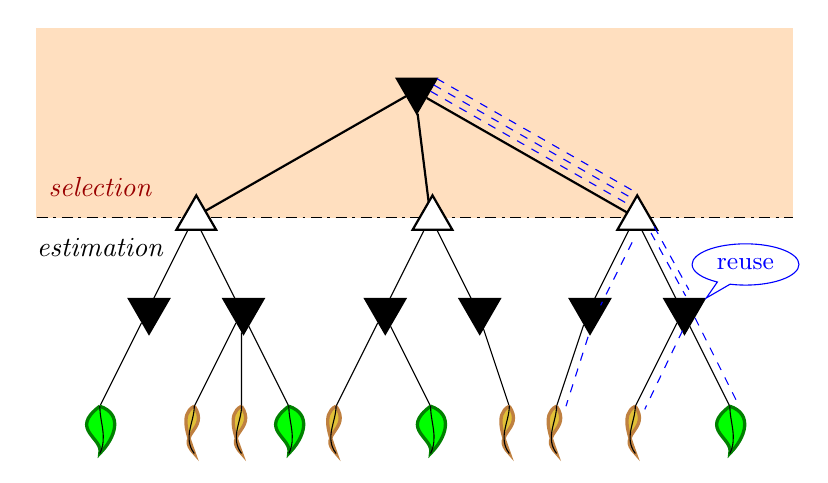
\begin{tikzpicture}
[node/.style={shape=isosceles triangle,isosceles triangle apex angle=60,
  thick},
black/.style={node,draw,fill=black,thick,rotate=30},
white/.style={node,draw,fill=white,thick,rotate=-30},
win/.style={node,shape=kite,draw=green!50!white,fill=green,below},
loss/.style={node,shape=kite,
            kite upper vertex angle=45,
            kite lower vertex angle=90,
            scale=0.75,
            draw=brown!50!black,fill=brown,below},
sample/.style={draw,thin,blue,dashed},
boundary/.style={dash pattern=on 4pt off 2pt on 1pt off 2pt}]
\begin{scope}[scale=0.8]
\draw [draw,fill,orange!25!white] (-6.0,1.0) rectangle (6.0,-2.0);
\draw[boundary] (-6.0,-2.0) -- (6.0,-2.0)
    (-5.0,-2.0) node [above=4pt,red!60!black] {\it selection}
    (-5.0,-2.0) node [below=4pt] {\it estimation};

\draw (0,0) node (root) [black] {};

\draw [thick] (root) -- ++(3.5,-2.0)
	node (s1) [white] {};
\draw [] (s1) -- ++( 0.75,-1.5)
	node (s11) [black] {}
        +(1.0,0.75) node [ellipse callout, callout absolute
        pointer={(s11.east)},draw,blue] {{\small reuse}};

\draw [] (s1) -- ++( -0.75,-1.5)
        node (s12) [black] {};
\draw [] (s11) -- ++( 0.75,-1.5)
        node (s111) {}; \win {(s111)};
\draw [] (s11) -- ++( -0.75,-1.5)
        node (s112) {}; \loss {(s112)};
\draw [] (s12) -- ++( -0.5,-1.5)
        node (s121) {}; \loss {(s121)};

\draw [thick] (root) -- ++(0.25,-2.0)
	node (s2) [white] {};
\draw [] (s2) -- ++( 0.75,-1.5)
	node (s21) [black] {};
\draw (s2) -- ++( -0.75, -1.5)
	node (s22) [black] {};
\draw [] (s21) -- ++( +0.5,-1.5)
	node (s211) {}; \loss {(s211)};
\draw (s22) -- ++( 0.75,-1.5)
	node (s221) {}; \win {(s221)};
\draw [] (s22) -- ++( -0.75,-1.5)
	node (s222) {}; \loss{(s222)};

\draw [thick] (root) -- ++(-3.5,-2.0)
	node (s3) [white] {};
\draw (s3) -- ++( 0.75,-1.5)
	node (s31) [black] {};
\draw [] (s3) -- ++( -0.75,-1.5)
	node (s32) [black] {};
\draw (s31) -- ++( 0.75,-1.5)
	node (s311) {}; \win {(s311)};
\draw [] (s31) -- ++( 0,-1.5)
	node (s312) {}; \loss {(s312)};
\draw  (s31) -- ++( -0.75,-1.5)
	node (s313) {}; \loss {(s313)};
\draw  [] (s32) -- ++( -0.75,-1.5)
	node (s321) {}; \win {(s321)};

% samples
\draw [sample] (0,0) ++(0.25,0.0) -- ++(3.15, -1.8)
                        ++(0.35,-0.45) -- ++(0.55, -1.0)
                        ++(-0.05,-0.55) -- ++(-0.6, -1.25);
\draw [sample] (0,0) ++(0.3,0.1) -- ++(3.15, -1.8)
                        ++(0.35,-0.45) -- ++(0.55, -1.0)
                        ++(0.1,-0.45) -- ++(0.65, -1.3);
\draw [sample] (0,0) ++(0.35,0.2)  -- ++(3.15, -1.8)
                     ++(-0.05, -0.8) -- ++(-0.5, -1.0)
                     ++(-0.2, -0.5) -- ++(-0.35, -1.1);
\end{scope}
\end{tikzpicture}
\end{frame}


\begin{frame}{Upper Bounds on Value of Information}
Assuming that:
\begin{enumerate}
\item Samples are i.i.d. given the value of the arm.
\item The expectation of a selection in a belief state is equal to the sample mean.
\end{enumerate}
Upper bounds on intrinsic VOI $\Lambda^b_i$ of testing the $i$th arm N
times are (based on Hoeffding inequality):
\begin{align*}
  \Lambda&_\alpha^b < \frac {N\overline X_\beta^{n_\beta}}
  {n_\alpha+1}\cdot 2\exp\left(- 1.37(\overline X_\alpha^{n_\alpha}\hspace{-0.5em} - \overline X_\beta^{n_\beta})^2 n_\alpha\right)\\
  \Lambda&_{i|i\ne\alpha}^b <  \frac {N(1-\overline
    X_\alpha^{n_\alpha})} {n_i+1}\cdot 2\exp\left(- 1.37(\overline X_\alpha^{n_\alpha}\hspace{-0.5em} - \overline X_i^{n_i})^2 n_i\right)
\end{align*}
Tighter bounds can be obtained (see the paper).
\end{frame}

\begin{frame}{VOI-based Sampling in Bernoulli Selection Problem}
25 arms, 10000 trials:
\begin{figure}[h]
\centering
\includegraphics[scale=0.65]{flat.pdf}
\end{figure}
UCB1 is always worse than VOI-aware policies (VOI, VOI+).
\end{frame}

\begin{frame}{Sampling in Trees}
\begin{itemize}
\item Hybrid sampling scheme:
\begin{enumerate}
\item At the {\it root node}: sample based on the VOI estimate.
\item At {\it non-root nodes}: sample using UCT.
\end{enumerate}
\item Stopping criterion: Assuming sample cost $c$ is known,\\
\hspace{1em}stop sampling when intrinsic VOI is less than $C=cN$:
\begin{align*}
\frac 1 N \Lambda_\alpha^b \le&\frac {\overline X_\beta^{n_\beta}}
  {n_\alpha+1}\Pr(\overline X_\alpha^{n_\alpha+N}\le\overline
  X_\beta^{n_\alpha})\le c\\
\frac 1 N \max_i\Lambda_i^b\le &\max_i\frac {(1-\overline X_\alpha^{n_\alpha})} {n_i+1}\Pr(\overline
  X_i^{n_i+N}\ge\overline X_\alpha^{n_\alpha})\le c\\
    &\forall i: i\ne\alpha
\end{align*}
\end{itemize}
\end{frame}

\begin{frame}{Sample Redistribution}
\begin{itemize}
\item The VOI estimate assumes that the information is {\bf discarded}
  between states.
\item MCTS {\bf re-uses rollouts} generated at earlier search states.
\vspace{\baselineskip}
\item Either incorporate `future' influence into the VOI estimate
  ({\it non-trivial!}).
\item Or behave myopically w.r.t. search tree depth:
\begin{enumerate}
\item Estimate VOI as though the information is discarded.
\item Stop early if the VOI is below a certain threshold.
\item Save the unused sample budget for search in future states.
\end{enumerate}
\item The cost $c$ of a sample  is\\\hspace{1em} the VOI of increasing a
  future budget by one sample.
\end{itemize}
\end{frame}

\begin{frame}{Playing Go Against UCT:\\\hspace{2em}Tuning the Sample Cost}
\begin{figure}[h]
  \centering
  \includegraphics[scale=0.65]{uctvoi.pdf}
\end{figure}
Best results for sample cost $c\approx 10^{-6}$:\\\hspace{2em}winning rate of {\bf
  64\%} for 10000 samples per ply.
\end{frame}

\begin{frame}{Playing Go Against UCT:
    \\\hspace{1em} Winning Rate vs. Number of Samples per Ply}

Sample cost $c$ fixed at $10^{-6}$:
\begin{figure}
  \centering
  \includegraphics[scale=0.65]{voi-wins.pdf}
\end{figure}
Best results for {\it intermediate} $N_{samples}$:
\begin{itemize}
\item When $N_{samples}$ is too low, poor moves are selected.
\item When $N_{samples}$ is too high, the VOI of further sampling
  is low.
\end{itemize}
\end{frame}

\section{Towards Rational Deployment of Multiple Heuristics in A*}


\begin{frame}
\frametitle{\visible<3->{Rational }\visible<2->{Lazy} $\astar$}

 %   Order the heuristics according to their simplcity\\
    Apply all heuristics to initial state $\init$\\
    Insert $\init$ into \OPEN \\
    \While{\OPEN~not empty}{
        $n$ $\gets$ best node from \OPEN \\
        \If{Goal(n)}{
            \Return trace(n)\\
        }
        \visible<2->{
        \If{$h_2$ was not applied to $n$ \visible<3->{ and $h_2$ is likely to pay off }}{
            Apply $h_2$ to $n$\\
            re-insert $n$ into \OPEN\\
            {\bf continue} ~~~~~~ //next node in OPEN\\
        }
        }
        \ForEach{child $c$ of $n$}{
            Apply $h_1$ to $c$\\
            insert $c$ into \OPEN\\
        }
        Insert $n$ into \CLOSED\\
    }
    \Return FAILURE

\end{frame}


\begin{frame}
\frametitle{Rational Decision}
\begin{itemize}
  \item When does computing $h_2$ pay off?
  \item Suppose $h_2$ was computed for state $s$. Then either:
  \begin{enumerate}
    \item $s$ will be expanded later on anyway
    \item an optimal goal is found before $s$ is expanded
  \end{enumerate}
  \item Computing $h_2$ pays off only in outcome 2 --- call this
  ``$h_2$ is helpful''
\end{itemize}

\begin{block}{}
\begin{quote}
``It is difficult to make predictions, especially about the future''
\vskip5mm
  \hspace*\fill{--- Yogi Berra / Neils Bohr}
\end{quote}
\end{block}

\end{frame}

\begin{frame}
\frametitle{Towards a Rational Decision}
\begin{itemize}
  \item Myopic assumption: this is the {\em last}
        meta-level decision to be made, and henceforth the algorithm
        will act like lazy $\astar$.
\item When a node re-emerges from the open list,
      compare the regret of computing $h_2$ as in lazy $\astar$, vs.
      just expanding the node.
\item Note: if rational lazy $\astar$ is indeed better than lazy
  $\astar$, the myopic assumption results in an upper bound
  on the regret.
\end{itemize}

\begin{center}
\begin{tabular}{|l|c|c|}
\hline
               & Compute $h_2$ & Bypass $h_2$\\
\hline
$h_2$ helpful &   0            & $\sim b(s) t_1 + (b(s) - 1)t_2$\\
\hline
$h_2$ not helpful & $\sim t_2$      & 0 \\
\hline
\end{tabular}\\
\vspace{3mm}
$b(s)$ denotes the number of successors of $s$\\
\vspace{3mm}
{\em Disclaimer: for the exact analysis, see the paper}
\end{center}
\end{frame}

\begin{frame}
\frametitle{From Regret to Rational Decision}
\begin{center}
\begin{tabular}{|l|c|c|}
\hline
               & Compute $h_2$ & Bypass $h_2$\\
\hline
$h_2$ helpful &   0            & $\sim b(s) t_1 + (b(s) - 1)t_2$\\
\hline
$h_2$ not helpful & $\sim t_2$      & 0 \\
\hline
\end{tabular}\\
\end{center}

\begin{itemize}
  \item Suppose that the probability of $h_2$ being helpful is $p_h$
  \item Then the rational decision is to compute $h_2$ iff:
  $$\frac{t_2}{t_1} < \frac {p_h b(s)} {1-p_h b(s)}$$  
\end{itemize}

\end{frame}


\begin{frame}
\frametitle{Approximating $p_h$}

$$\frac{t_2}{t_1} < \frac {p_h b(s)} {1-p_h b(s)}$$

\begin{itemize}
  \item We can directly measure $t_1, t_2$ and $b(s)$, but need to approximate $p_h$
  \item If $s$ is a state at which $h_2$ was helpful, then we computed
  $h_2$ for $s$, but did not expand $s$. Denote the number of such states by
  $B$.
  \item Denote by $A$ the number of states for which we computed $h_2$.
  \item We can use $\frac{A}{B}$ as an estimate for $p_h$
  \item To get an estimate which is more stable, we use a weighted average with
  $k$ fictitious examples giving an estimate of $p_{init}$: 
  $$\frac{(A + p_{init} \cdot k)}{B + k}$$
  \item We use $p_{init} = 0.5$ and $k = 1000$
\end{itemize}

\end{frame}

\begin{frame}
\frametitle{Empirical Evaluation: Weighted 15 Puzzle}

\begin{itemize}
  \item $h_1$ --- weighted manhattan distance
  \item $h_2$ --- lookahead to depth $l$ with $h_1$
\end{itemize}

\begin{tabular}{|l|r|r|r||r|r|r|}
\hline
    & \multicolumn{3}{|c|}{Generated } & \multicolumn{3}{|c|}{Time }\\
$l$ &	 $\astar$ & \lazyastar & \rationallazyastar &	 $\astar$ & \lazyastar
& \rationallazyastar\\
\hline
2 	& 1,206,535 & 	 1,206,535 &	 1,309,574 &	 0.707 & 	 0.820& 	 0.842 \\ 
\hline
4 	& 1,066,851 & 	 1,066,851 &	 1,169,020 &	 0.634 &	 0.667& 	 0.650 \\ 
\hline
6 	& 889,847 &	 889,847 &	 944,750 &	 {\bf 0.588} &	 0.533 &	 0.464 \\ 
\hline
8 	& 740,464 &	 740,464 &	 793,126 &	 0.648 &	 {\bf 0.527} &	 0.377 \\ 
\hline
10 	& 611,975 &	 611,975 &	 889,220 &	 0.843 &	 0.671 	& {\bf 0.371} \\ 
\hline
12 	& {\bf 454,130} &	 {\bf 454,130} &	 807,846 &	 0.927 &	 0.769 &	 0.429 \\
\hline
\end{tabular}

\end{frame}

\begin{frame}
\frametitle{Empirical Evaluation: Planning Domains}

\begin{itemize}
  \item $h_{LA}$ --- admissible landmarks
  \item $\lmcut$ --- landmark cut
\end{itemize}

\begin{tabular}{|l|r||r|r|r|}
\hline
    &         & \multicolumn{3}{|c|}{623 Commonly Solved}\\
Alg &  Solved & Time (GM) &  Expanded & Generated\\
\hline
$h_{LA}$ & 	 698 &	 1.18 & 183,320,267 & 1,184,443,684\\
 $\lmcut$ &	 697 &	 0.98 & 23,797,219 & 114,315,382\\
 max &	 722 &	 0.98 & \textbf{22,774,804} & \textbf{108,132,460}\\ 
 selmax &	 747 & 	 0.89 & 54,557,689 & 193,980,693\\
\hline 
 \lazyastar	& 747 &	 0.79 & \textbf{22,790,804} & \textbf{108,201,244}\\
 \rationallazyastar &	 \textbf{750} &	 \textbf{0.77} & 25,742,262 &
 110,935,698\\
\hline 
\end{tabular}

\begin{itemize}
  \item \rationallazyastar~solves the most problems, and is fastest on average
\end{itemize}
\end{frame}


\section{Insights into the Methodology}
\begin{frame}
\frametitle{Insights into the Methodology}
\begin{itemize}
\item Rational metareasoning works best when:
\begin{enumerate}
\item Ubiquitous heuristic evaluation of the search space \emph{decreases} the total search
  time.
\item The heuristic computation time constitutes \emph{a significant part} of
  the total search time. 
\end{enumerate}
\item It is important to identify the right metareasoning decision.
\item Simple utility and information model serve well.
\item Tunable parameters should reflect algorithm implementation
  rather than problem set.
\end{itemize}
\end{frame}

\section{Summary and Future Work}
\begin{frame}
\frametitle{Summary and Future Work}

Novel techniques:
\begin{itemize}
\item ``Rational Deployment of heuristics in CSP'' demonstrated
  derivation of the belief model from the algorithm rather than
  problem set.
\item ``VOI-aware Monte-Carlo tree search''
provided distribution-independent upper bounds for semi-myopic VOI
estimates in Monte-Carlo sampling.
\item ``Towards rational deployment of Multiple
Heuristics in A*'', introduced a novel area of application of rational
metareasoning---optimal search in optimization problems.
\end{itemize}

Future research:
\begin{itemize}
\item Whether a dramatic breakthrough in performance is possible.
\item Rational metareasoning when action costs and state utilities are
  not commensurable.
\end{itemize}

\end{frame}

\begin{frame}
\begin{center}
\begin{huge}
Thank You
\end{huge}
\end{center}
\end{frame}

\end{document}
